\subsubsection{Overview}

The \textbf{RollupX Prototype Prover} is a \textbf{zk-Rollup (Zero-Knowledge Rollup)} scaling solution for Ethereum. Its primary purpose is to enable \textbf{low-gas transfers of ETH and ERC-20 tokens} by moving transaction execution off-chain (Layer 2) while preserving the security guarantees of the Ethereum mainnet (Layer 1) through \textbf{cryptographic validity proofs}.

The core idea is simple: instead of processing every transaction on Ethereum directly, transactions are batched off-chain into \textbf{blocks}, a \textbf{zero-knowledge proof} is generated to attest to the correctness of all those transactions, and only the compact proof plus a small amount of public data is submitted on-chain. The Ethereum smart contract verifies the proof and updates the state without re-executing the transactions.

The system uses a \textbf{PLONK} proof system as an universal, succinct, non-interactive argument of knowledge (SNARK) backed by \textbf{Kate/KZG polynomial commitments} over the BN256 elliptic curve.

\subsubsection{System Components (Broad View)}

The system consists of three principal components that interact to form the full rollup pipeline:

\paragraph{Rollup Smart Contract (L1  Solidity)}

Located in \texttt{contracts/contracts/rollup.sol} and \texttt{contracts/contracts/PlonkCore.sol}, this is the on-chain anchor. It:
\begin{itemize}
    \item Manages user \textbf{balances} and \textbf{account state} on Ethereum.
    \item Accepts \textbf{priority operations} from L1 (e.g., \texttt{Deposit}, \texttt{FullExit}).
    \item \textbf{Commits} blocks by verifying their data integrity and storing block hashes.
    \item \textbf{Verifies PLONK proofs} (both single and recursive/aggregated) submitted by the server.
    \item \textbf{Executes} proven blocks to finalise withdrawals and state changes.
\end{itemize}

\paragraph{Server Application (L2  Rust)}

The server is the L2 node that orchestrates the rollup network. It exists in monolithic (\texttt{core/bin/server}) or microservice form:

\begin{table}[h]
\centering
\begin{tabular}{lll}
\toprule
\textbf{Microservice} & \textbf{Path} & \textbf{Responsibility} \\
\midrule
\textbf{Core} & \texttt{core/bin/Rollup\_core} & Mempool management,block generate \\
\textbf{API} & \texttt{core/bin/Rollup\_api} & REST API \& JSON RPC (HTTP) \\
\textbf{Ethereum Sender} & \texttt{core/bin/Rollup\_eth\_sender} & Submits prove/execute tx to L1 \\
\textbf{Witness Generator} & \texttt{core/bin/Rollup\_witness\_generator} & Builds circuit witness data;prover API \\
\bottomrule
\end{tabular}
\end{table}

\paragraph{Prover Application (Off-chain Worker Rust)}

Located in \texttt{core/bin/prover}, the prover is the computationally-intensive worker that generates zk-SNARK proofs. It polls the server for jobs, generates proofs, and returns results. Multiple provers can run concurrently for horizontal scalability.

\subsubsection{Transaction Lifecycle : Step-by-Step}

The following outlines how a transaction flows through the system from submission to finality:

\begin{verbatim}
 User submits Tx (L2)
        |
        |
        |
        v
┌──────────────────┐
│   Server (Core)   │         ← Accepts tx, validates, adds to mempool
│  Block Assembly   │         ← Groups txs into a block (with pubdata)
└──────────────────┘
        |
        |
        |
        v
┌──────────────────────────┐
│   Witness Generator       │ ← Builds circuit witness (account tree + ops)
│  (Prover Server API)     │  ← Stores witness in DB, serves it to provers
└──────────────────────────┘
        |
        |
        |
        v
┌──────────────────────────┐
│   Prover Worker           │ ← Polls for job, receives witness
│  (PlonkStepByStepProver) │  ← Generates PLONK single proof
│                          │  ← Generates aggregated recursive proof
└──────────────────────────┘
        |
        | 
        |
        v
┌──────────────────────────┐
│   Ethereum Sender         │ ← commitBlocks() → proveBlocks() → executeBlocks()
│  → L1 Smart Contract     │  ← On-chain verification via PlonkCore.sol
└──────────────────────────┘
\end{verbatim}

\textbf{Step 1 --- Transaction Submission:} Users submit L2 transactions (\texttt{Transfer}, \texttt{Withdraw}, \texttt{ChangePubKey}, \texttt{ForcedExit}) or trigger L1 priority operations (\texttt{Deposit}, \texttt{FullExit}).

\textbf{Step 2 --- Block Assembly:} The server's Core service batches transactions into blocks, applying state changes to the account tree.

\textbf{Step 3 --- Witness Generation:}  The Witness Generator loads the circuit account tree, applies each operation to build the \textbf{circuit witness} data, and stores it in the database.

\textbf{Step 4 --- Proof Generation:}  A Prover worker fetches the witness, generates a PLONK single proof per block, then aggregates proofs using a recursive circuit.

\textbf{Step 5 --- On-chain Finalization:}  The Ethereum Sender commits the block data on-chain, submits the aggregated proof, and upon successful verification the block is executed (withdrawals processed, state finalized).

\begin{figure}[htbp]
    \centering
    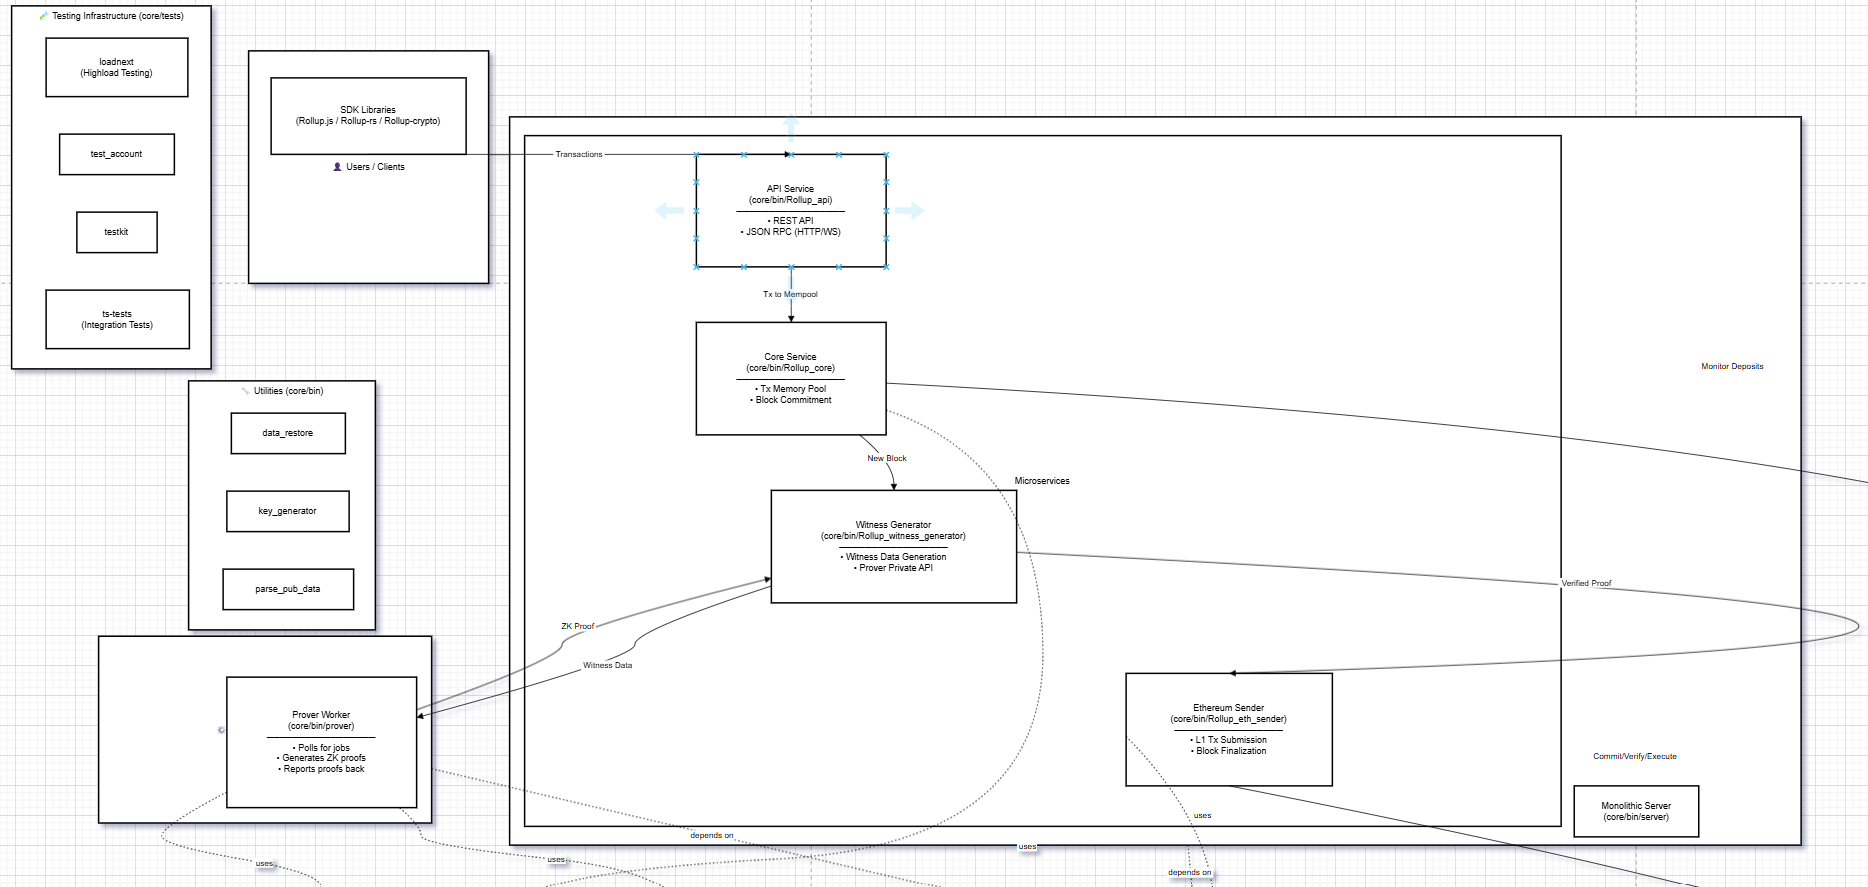
\includegraphics[width=0.9\textwidth]{figures/Diagram -1.png}
\end{figure}
\begin{figure}[htbp]
    \centering
    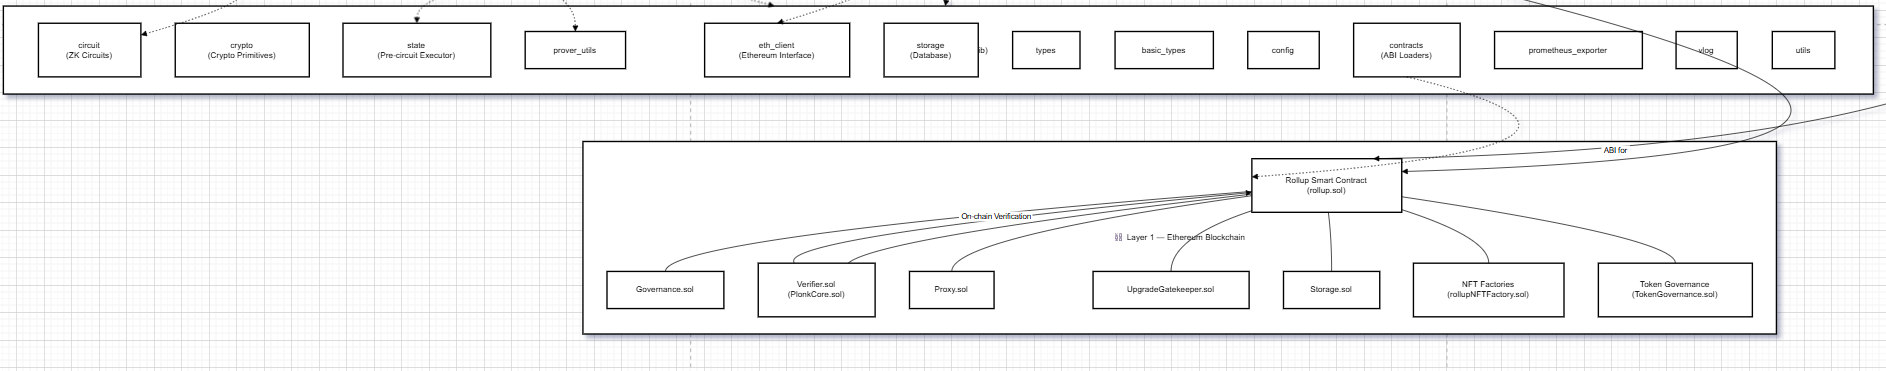
\includegraphics[width=0.9\textwidth]{figures/Daiagram -2.png}
    \caption{RollupX Prover Architecture showing the interaction between 
             Witness Generator, Prover Worker, and Ethereum contracts}
    \label{fig:prover-architecture}
\end{figure}

\subsubsection{The Prover --- Deep Dive}

\paragraph{Architecture \& Traits}

The prover system is built around two key Rust traits defined in \texttt{core/bin/prover/src/lib.rs}:

\begin{lstlisting}[caption={Core prover traits from \texttt{core/lib/prover\_utils/src/lib.rs}}]
/// Trait that provides type needed by prover to initialize.
pub trait ProverConfig {
    fn from_env() -> Self;
}

/// Trait that tries to separate prover from networking (API)
pub trait ProverImpl {
    type Config: ProverConfig;
    fn create_from_config(config: Self::Config) -> Self;
    fn get_request_aux_data(&self) -> ProverInputRequestAuxData { ... }
    /// Resource heavy operation
    fn create_proof(&self, data: JobRequestData) -> anyhow::Result<JobResultData>;
}
\end{lstlisting}

This trait-based design decouples proof logic from networking, allowing two interchangeable implementations:

\begin{table}[h]
\centering
\begin{tabular}{lll}
\toprule
\textbf{Implementation} & \textbf{File} & \textbf{Purpose} \\
\midrule
\texttt{PlonkStepByStepProver} & \texttt{core/bin/prover/src/plonk\_step\_by\_step\_prover.rs} & PLONK proofs \\
\texttt{DummyProver} & \texttt{core/bin/prover/src/dummy\_prover.rs} & Testing prover --- returns precomputed proofs \\
\bottomrule
\end{tabular}
\end{table}

\paragraph{Prover Work Cycle}

The main event loop is in \texttt{prover\_work\_cycle} (\texttt{core/bin/prover/src/lib.rs}):

\begin{enumerate}
    \item \textbf{Register} with the server via the API client.
    \item \textbf{Poll} the server's Witness Generator API (\texttt{get\_job}) for an idle prover job.
    \item \textbf{Receive} either a \texttt{BlockProof} job (single block witness) or an \texttt{AggregatedBlockProof} job (multiple single proofs to aggregate).
    \item \textbf{Compute} the proof on a blocking thread (via \texttt{compute\_proof\_no\_blocking}).
    \item \textbf{Send heartbeats} concurrently to keep the job alive while computing.
    \item \textbf{Publish} the result back to the server (\texttt{publish} endpoint).
    \item Repeat until shutdown.
\end{enumerate}

\vspace{5mm}
\paragraph{Prover Components}

The prover's internal components span multiple crates:

\subparagraph{Circuit (\texttt{core/lib/circuit})}

Defines the \textbf{ZkSyncCircuit} --- the arithmetic circuit that enforces transaction correctness. Key elements:

\begin{itemize}
    \item \textbf{\texttt{ZkSyncCircuit}} (\texttt{core/lib/circuit/src/circuit.rs}): The main circuit implementing \texttt{Circuit<E>}. It synthesizes constraints for every operation in a block, with a single public input: the \texttt{pub\_data\_commitment}.
    \item \textbf{\texttt{Witness} trait} (\texttt{core/lib/circuit/src/witness/mod.rs}): Each operation type (Deposit, Transfer, Withdraw, etc.) implements this trait to generate witness data by applying the operation to a \texttt{CircuitAccountTree}.
    \item \textbf{Operation-specific witnesses} (\texttt{core/lib/circuit/src/witness/\{deposit, transfer, withdraw, ...\}.rs}): Implements state transition logic for each zkSync operation.
\end{itemize}

\subparagraph{Crypto Primitives (\texttt{core/lib/crypto})}

Cryptographic foundations:

\begin{itemize}
    \item \textbf{Proof types} (\texttt{core/lib/crypto/src/proof.rs}): Defines \texttt{SingleProof} (PLONK proof for one block) and \texttt{AggregatedProof} (recursive proof aggregating multiple single proofs), along with their encoded/serialized forms for on-chain submission.
    \item \textbf{BN256 elliptic curve} operations, Rescue hash functions, and EdDSA signature verification.
\end{itemize}

\subparagraph{Prover Utils (\texttt{core/lib/prover\_utils})}

The engine room for proof generation:

\begin{itemize}
    \item \textbf{\texttt{SetupForStepByStepProver}} (\texttt{core/lib/prover\_utils/src/lib.rs}): Prepares the PLONK proving setup:
\end{itemize}

\begin{lstlisting}[language=Rust,caption={Setup structure from \texttt{core/lib/prover\_utils/src/lib.rs}}]
pub struct SetupForStepByStepProver {
    setup_polynomials: SetupPolynomials<Engine, PlonkCsWidth4WithNextStepParams>,
    hints: Vec<(usize, TranspilationVariant)>,
    setup_power_of_two: u32,
    key_monomial_form: Option<Crs<Engine, CrsForMonomialForm>>,
}
\end{lstlisting}

\begin{itemize}
    \item \textbf{\texttt{PlonkVerificationKey}}: Reads and caches per-block-size verification keys.
    \item \textbf{\texttt{aggregated\_proofs}} module (\texttt{core/lib/prover\_utils/src/aggregated\_proofs.rs}): Handles recursive proof aggregation.
\end{itemize}

\paragraph{Key Generator (\texttt{core/bin/key\_generator})}

A one-time utility that generates:

\begin{itemize}
    \item PLONK verification keys for each supported block size.
    \item Recursive aggregation verification keys.
    \item Sample/precomputed proofs for testing.
    \item The on-chain \textbf{Verifier contract} (auto-generated Solidity with embedded VKs).
\end{itemize}

\paragraph{How Proof Generation Works}
\paragraph{Step A --- Setup Preparation}

The prover prepares the PLONK proving setup by transpiling the circuit, computing setup polynomials, and loading the Common Reference String.


\begin{lstlisting}[caption={Setup preparation from \texttt{core/lib/prover\_utils/src/lib.rs}}]
impl SetupForStepByStepProver {
    pub fn prepare_setup_for_step_by_step_prover<C: Circuit<Engine> + Clone>(
        circuit: C,
        download_setup_file: bool,
    ) -> Result<Self, anyhow::Error> {
        let hints = transpile(circuit.clone())?;           // Transpile circuit to PLONK gates
        let setup_polynomials = setup(circuit, &hints)?;   // Compute setup polynomials
        let size = setup_polynomials.n.next_power_of_two().trailing_zeros();
        let setup_power_of_two = std::cmp::max(size, SETUP_MIN_POW2);
        let key_monomial_form = Some(get_universal_setup_monomial_form(
            setup_power_of_two, download_setup_file,
        )?);                                                // Load CRS (trusted setup)
        Ok(SetupForStepByStepProver { setup_polynomials, hints, setup_power_of_two, key_monomial_form })
    }
}
\end{lstlisting}

\begin{enumerate}
    \item \textbf{Transpile} the circuit into a PLONK-compatible gate representation (width-4 with next-step parameters).
    \item \textbf{Compute setup polynomials} (selector/permutation polynomials from the constraint system).
    \item \textbf{Load the CRS} (Common Reference String / Universal Setup) in monomial form from disk or network (power of two ranges from $2^{20}$ to $2^{26}$).
\end{enumerate}

\paragraph{Step B --- Single Proof Generation}

A single PLONK proof is generated for one block using the prepared setup, with immediate self-verification before returning the proof.

\begin{lstlisting}[caption={Single proof generation from \texttt{core/lib/prover\_utils/src/lib.rs}}]
pub fn gen_step_by_step_proof_using_prepared_setup<C: Circuit<Engine> + Clone>(
    &self, circuit: C, vk: &PlonkVerificationKey,
) -> Result<SingleProof, anyhow::Error> {
    let rns_params = RnsParameters::<Engine, <Engine as EngineTrait>::Fq>::new_for_field(68, 110, 4);
    let rescue_params = Bn256RescueParams::new_checked_2_into_1();
    let transcript_params = (&rescue_params, &rns_params);
    let proof = prove_by_steps::<_, _, RescueTranscriptForRNS<Engine>>(
        circuit.clone(), &self.hints, &self.setup_polynomials,
        None, self.key_monomial_form.as_ref().unwrap(), Some(transcript_params),
    )?;
    let valid = verify::<_, _, RescueTranscriptForRNS<Engine>>(&proof, &vk.0, Some(transcript_params))?;
    anyhow::ensure!(valid, "proof for block is invalid");
    Ok(proof.into())
}
\end{lstlisting}

\begin{enumerate}
    \item \textbf{\texttt{prove\_by\_steps}}: Executes the PLONK prover algorithm using a Rescue-based Fiat-Shamir transcript. This produces wire commitments, the grand product polynomial, quotient polynomial commitments, and opening proofs at evaluation points $z$ and $z\omega$.
    \item \textbf{\texttt{verify}}: Immediately self-validates the proof against the verification key before returning it --- ensuring no invalid proofs are published.
\end{enumerate}

\subparagraph{Step C --- Proof Aggregation (Recursive SNARKs)}

Multiple single proofs are combined into one \textbf{aggregated proof} via a recursive aggregation circuit:

\begin{lstlisting}[language=Rust,caption={Aggregated proof generation from \texttt{core/lib/prover\_utils/src/aggregated\_proofs.rs}}]
pub fn gen_aggregate_proof(...) -> anyhow::Result<AggregatedProof> {
    let aggregate = create_zksync_recursive_aggregate(
        RECURSIVE_CIRCUIT_VK_TREE_DEPTH, RECURSIVE_CIRCUIT_NUM_INPUTS,
        &single_vks, &proofs, &vk_indexes, &g2_bases,
    )?;
    let setup = create_recursive_circuit_setup(proofs.len(), ...)?;
    let rec_aggr_proof = proof_recursive_aggregate_for_zksync(
        ..., &single_vks, &proofs, &vk_indexes, &vk_for_recursive_circuit,
        &setup, &universal_setup, true, &worker,
    )?;
    // Verify the recursive proof
    let is_valid = verify(&vk_for_recursive_circuit, &rec_aggr_proof, None)?;
    Ok(AggregatedProof { proof: rec_aggr_proof, individual_vk_inputs, individual_vk_idxs, aggr_limbs })
}
\end{lstlisting}

This creates a SNARK-of-SNARKs: a single proof that attests to the validity of all individual block proofs. The on-chain verifier (\texttt{PlonkCore.sol}) calls \texttt{verify\_recursive()} which reconstructs the recursive public input and performs a final pairing check.

\subparagraph{Step D --- On-Chain Verification}

The Solidity contract \texttt{PlonkCore.sol} implements both:
\begin{itemize}
    \item \textbf{\texttt{verify()}} --- standard PLONK verification with pairing check.
    \item \textbf{\texttt{verify\_recursive()}} --- combines inner (aggregated) and outer (recursive circuit) pairing elements, then verifies with a single \texttt{pairingProd2} call.
\end{itemize}

\paragraph{Proof Job Types}

The prover handles two job types, tracked via \texttt{ProverJobStatus} (Idle $\rightarrow$ InProgress $\rightarrow$ Done):

\begin{table}[h]
\centering
\begin{tabular}{lll}
\toprule
\textbf{Job Type} & \textbf{Priority} & \textbf{Description} \\
\midrule
\texttt{SingleProof} & 1 (higher) & Prove one block's circuit \\
\texttt{AggregatedProof} & 0 (lower) & Aggregate N single proofs into one recursive proof \\
\bottomrule
\end{tabular}
\end{table}

\paragraph{Caching \& Optimisation}

\begin{itemize}
    \item \textbf{\texttt{PreparedComputations} cache}: The \texttt{PlonkStepByStepProver} caches setup data per block size. If consecutive blocks have the same chunk size, the expensive transpilation/setup step is skipped.
    \item \textbf{\texttt{UNIVERSAL\_SETUP\_CACHE}}: A global lazy-static cache for CRS monomial forms, preventing repeated disk reads of large setup files.
    \item The \texttt{DummyProver} provides precomputed proofs for development/testing, eliminating the multi-minute proof generation time.
\end{itemize}

\subsubsection{Supported Operations}

The circuit enforces correctness for all zkSync operation types:

\begin{table}[h]
\centering
\begin{tabular}{lll}
\toprule
\textbf{Category} & \textbf{Operations} & \textbf{Enum} \\
\midrule
\textbf{L2 Transactions} & \texttt{Transfer}, \texttt{Withdraw}, \texttt{ChangePubKey}, \texttt{ForcedExit}, \texttt{Swap}, \texttt{MintNFT}, \texttt{WithdrawNFT} & \texttt{ZkSyncTx} \\
\textbf{L1 Priority Ops} & \texttt{Deposit}, \texttt{FullExit} & \texttt{ZkSyncPriorityOp} \\
\textbf{Combined} & All of the above (with block metadata) & \texttt{ZkSyncOp} \\
\bottomrule
\end{tabular}
\end{table}

\subsubsection{Conclusion} 

The \textbf{RollupX Prototype Prover} implements a complete zk-Rollup proving pipeline based on the PLONK zero-knowledge proof system. The architecture cleanly separates concerns: the \textbf{Witness Generator} transforms executed blocks into arithmetic circuit inputs, the \textbf{Prover} generates PLONK proofs using a step-by-step algorithm with setup caching for efficiency, and a \textbf{recursive aggregation circuit} compresses multiple block proofs into a single succinct proof for on-chain verification. The Ethereum smart contract finalises state transitions by verifying these aggregated proofs via elliptic curve pairing checks. \vspace{5mm} \\

The design demonstrates several key properties desirable in an academic context: \textbf{modularity} (trait-based prover abstraction allowing real vs. dummy implementations), \textbf{scalability} (horizontal prover scaling via a job-queue architecture), and \textbf{correctness} (every generated proof is self-verified before submission). The use of universal PLONK setups (CRS powers $2^{20}$--$2^{26}$) avoids per-circuit trusted ceremonies, and the recursive proof aggregation minimises L1 gas costs by amortising verification across multiple blocks in a single pairing operation.